\section{Using external devices \label{sec:external}}

Our third and last approach was to use external devices to compute the context switching time.
In this way, all the heavy computational processes are done outside of the board but in a computer, for example.

\subsection{Choice of the external device}

Our first idea was to implement it with Python3.7 on a desktop computer.
Using the UART protocol over USB, the board sends a single byte containing the thread ID that is read by a Python script on the computer.

The motivations for using this alternative are:
\begin{itemize}
  \item Sending one byte of data over USB with UART have a smaller impact than computing the context switching time locally on the board;
  \item Heavy computational tasks of the framework are done on the computer and not on the board;
  \item Using Python3.7, we can achieve a time precision at the nanosecond.
\end{itemize}

However, after discussing with the embedded community, we abandonned this idea for the following reasons.
There is buffering happening on the USB-serial chip on the board, on the PC's USB hardware, in the PC USB-serial driver and also in the desktop operating systems.
Those buffering will add delay in our measurements.
Context switchs will occur on the desktop computer that will invalidate any timing value.

Instead, we decided to use a device called the Pocket Science Lab to perform our experiment.

\begin{figure}[!ht]
  \centering
  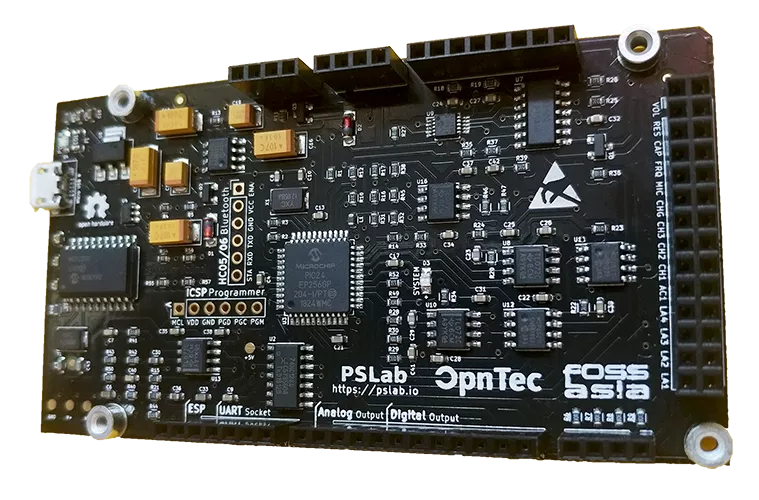
\includegraphics[scale=0.25]{assets/pslab.png}
  \caption{\label{fig:pslab}Pocket Science Lab device from \href{https://pslab.io}{PSLab.io}}
\end{figure}

The Pocket Science Lab device from \href{https://pslab.io}{PSLab.io} comes with a built-in 4-Channel up to 2MSPS oscilloscope, multimeter, 4-Channel, 4 MHz logic analyser, and other digital instruments.
Using the Python librairy \href{https://github.com/fossasia/pslab-python}{pslab-python}, we can communicate with the board and experiment with it.
With a device like the PSLab, we can left the benchmarked board that contains our simple application untouched in terms of heavy computations.

\subsection{Roles of the devices}

With the benchmarked board, the PSLab and the computer, we have three devices that we use to compute the context switching time.
The figure \ref{fig:external-benchmarking-framework-schema} shows the connections between the different devices.
To make some clarity, we have defined a specific role to each device.

\subsubsection{The benchmarked board}
The benchmarked board runs the RTOS of our choice with our benchmarking framework and our simple application.
It communicate with our computer through UART and with the PSLab using a single GPIO.
Its role is to simply run the application and change the state of the GPIO depending on the tasks status.

\subsubsection{The computer}
The computer is the brain of the benchmarking framework.
It is responsible of communicating with both the benchmarked board and the PSLab through the UART protocol.
It is its responsability to coordinate the benchmarked board and the PSLab in order to retrieve the context switching time.
The computer is also the place where all the data are accumulated.

\subsubsection{The PSLab}
Connected with a single GPIO to the benchmarked board, the PSLab watch for any context switch.
It measure the context switching time using its logical analyser.
The board receives its instruction and send the measures through UART with our computer.

\begin{figure}[!ht]
  \centering
  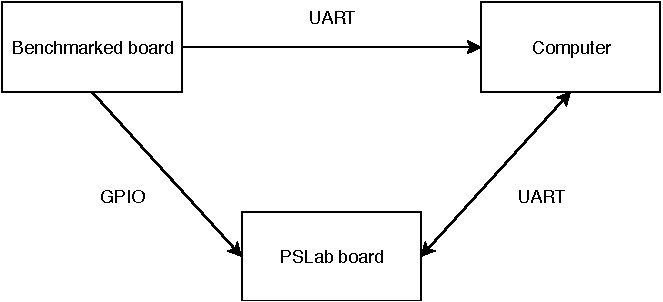
\includegraphics[scale=1]{assets/external-benchmarking-framework-schema.pdf}
  \caption{\label{fig:external-benchmarking-framework-schema}Interaction schema of the devices used in the framework}
\end{figure}

\subsection{Usage of the Pocket Science Lab}

The PSLab will monitor a single GPIO and measure the context switching time from it.
The figure \ref{fig:external-framework-context-switching-time-measurement} shows the steps in the measurement with the PSLab.
Each task will set the GPIO up at the start of its execution and then reset the GPIO once it ended.
In our example, the task 1 set up the GPIO at the step A and the GPIO is in high position at step A'.
Once the task 1 is finished, it reset the GPIO at the step B that will be in position at step B'.
The same process occurs for the task 2.
The task 2 set up the GPIO at step C.
The GPIO is in high position at step C'.
Finally, the task 2 reset the GPIO at the end of its execution at step D and the GPIO will be in position low at step D'.
From our measurements made with the reference value, we know that the rising time of the GPIO is around 10 nanoseconds so it can be omitted.

\begin{figure}[!ht]
  \centering
  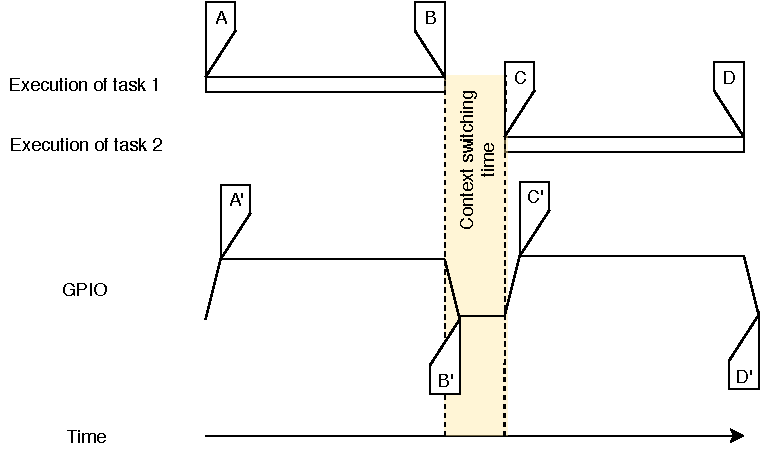
\includegraphics[scale=1]{assets/external-framework-context-switching-time-measurement.pdf}
  \caption{\label{fig:external-framework-context-switching-time-measurement}Measurement of the context switching time with a single GPIO}
\end{figure}

\subsection{Using the framework with our simple application}

To understand the framework implementation, it is important to understand what happens when our simple application boots.
But both from the point of view of the benchmarked board and from the point of view of the PSLab and the computer.

\subsubsection{Point of view of the benchmarked board}
When the application boots, it will initialize the framework.
An initializiation is required to use the GPIO.
Once the initializiation is done, the first task starts.
It will call \texttt{bench\_on()} from the framework.
In the framework-space, \texttt{bench\_on()} will have for effect to set the GPIO up.
When the task is done, it will call \texttt{bench\_off()} that will reset the GPIO.
The second task goes in the foreground and will also call \texttt{bench\_on()} and, latter, \texttt{bench\_off()}.

\subsubsection{Point of view of the PSLab and the computer}
The PSLab will listen for an interval between a falling and a rising edge.
In the figure \ref{fig:external-framework-context-switching-time-measurement}, this interval happens between the step B' and C'.
For reminder, the rising time can be omitted.
Once the PSLab detect an interval, it compute its time.
This interval time is the context switching time.
This measure is send to the computer that will store it.

\subsection{Framework implementation}

The interaction between the benchmarked board and the PSLab is done through a GPIO that is controlled by the benchmarked board.
The code in the benchmarked board is quite straightforward.
First, our simple application need initialize the framework and start its tasks.
Then, we need to add \texttt{bench\_on()} and \texttt{bench\_off()} respectively at the start and at the end of the two tasks.
The code of the updated application is shown in the listing \ref{lst:external-app-code}.

\begin{lstlisting}[style=CStyle, float, caption={Source code of the simple application in Contiki}, label={lst:external-app-code}]
#include "contiki.h"
#include "sys/clock.h"
#include "bench-context-switching.h"

#include <stdio.h>

PROCESS(init_task, "Init task");
PROCESS(task_1, "First task");
PROCESS(task_2, "Second task");
AUTOSTART_PROCESSES(&init_task);

PROCESS_THREAD(init_task, ev, data)
{
    PROCESS_BEGIN();

    bench_init();

    process_start(&task_1, NULL);
    process_start(&task_2, NULL);

    PROCESS_END();
}

PROCESS_THREAD(task_1, ev, data)
{
    PROCESS_BEGIN();

    while (1)
    {
        bench_on();
        clock_delay_usec(1000);
        bench_off();
        PROCESS_PAUSE();
    }

    PROCESS_END();
}

// ...
// task_2 is identical to task_1
\end{lstlisting}

During the initializiation, the framework will setup the GPIO as an output port. The listing \ref{lst:external-init-code} shows this process.
The \texttt{bench\_on()} and \texttt{bench\_off()} will just set or reset the GPIO like shown in the listing \ref{lst:external-on-off-code}.

\begin{lstlisting}[style=CStyle, caption={Initializiation of the framework in Contiki}, label={lst:external-init-code}]
void bench_init()
{
    GPIO_SOFTWARE_CONTROL(GPIO_PORT_TO_BASE(GPIO_C_NUM), GPIO_PIN_MASK(2));
    GPIO_SET_OUTPUT(GPIO_PORT_TO_BASE(GPIO_C_NUM), GPIO_PIN_MASK(2));
}
\end{lstlisting}

\begin{lstlisting}[style=CStyle, caption={\texttt{bench\_on()} and \texttt{bench\_off()} implementation in Contiki}, label={lst:external-on-off-code}]
void bench_on(uint32_t pid)
{
    GPIO_SET_PIN(GPIO_PORT_TO_BASE(GPIO_C_NUM), GPIO_PIN_MASK(2));
}

void bench_off()
{
    GPIO_CLR_PIN(GPIO_PORT_TO_BASE(GPIO_C_NUM), GPIO_PIN_MASK(2));
}
\end{lstlisting}

Finally, from the computer, we need to retrieve and store the interval measurement from the PSLab.
To do so, we use a Python script shown in listing \ref{lst:python-pslab} that connect to the PSLab and retrieve the context switching time between a falling and a rising edge.

\begin{lstlisting}[style=CStyle, language=python, caption={Python script to communicate with the PSLab and retrieve the interval measurement}, label={lst:python-pslab}]
from PSL import sciencelab
I = sciencelab.connect()

VALUES = []

while True:
    CS_TIME = I.MeasureInterval('ID1', 'ID1', 'falling', 'rising')
    VALUES.append(CS_TIME)
\end{lstlisting}


% In order to implement this third approach, we need to update our simple task, create our framework in Contiki as an app and creating a Python script that will run on the computer and communicate with both the benchmarked board and the PSLab.

% \subsubsection{Protocol}

% We first need to define some sort of protocol to communicate between our three devices.
% The figure \ref{fig:external-protocol} shows the interactions between every device.

% \begin{figure}[!ht]
%   \centering
%   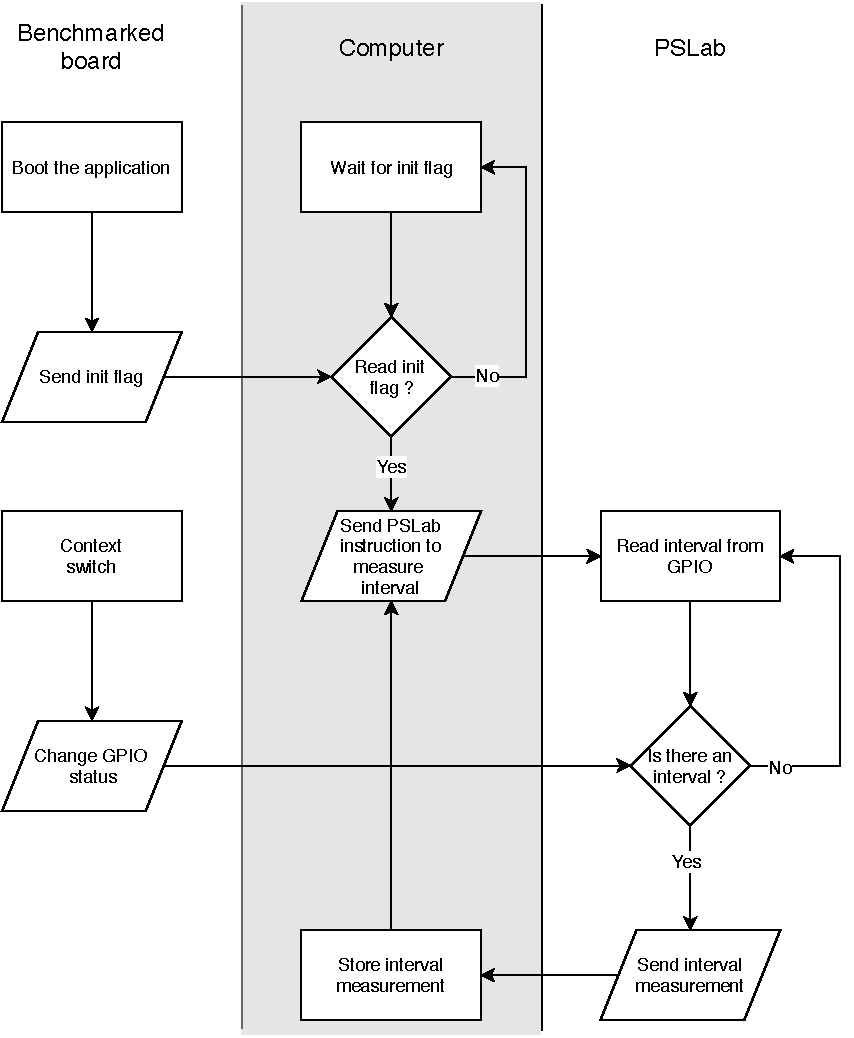
\includegraphics[scale=0.7]{assets/external-protocol.pdf}
%   \caption{\label{fig:external-protocol}Schema of the protocol used between the devices}
% \end{figure}

% The first step is to start the Python script on the computer. It will read all the messages send by the board on the UART port.
% When the benchmarked board boots, it will send an init flag to the computer once its GPIO is setup and it is ready to transmit information through the GPIO.
% Once the computer read the init flag, it will send to the PSLab the instruction to read a time interval between a falling and a rising edge like shown in the figure \ref{fig:external-framework-context-switching-time-measurement}.
% Once a task is done in the benchmarked board, it will reset the GPIO that will trigger the PSLab measurement.
% This measurment is send to the computer and the computer will save the value.
% The computer will then send the instruction to the PSLab again and wait for a new measurement.

% \subsubsection{Python script}

% The Python script that run on the computer is the coordinator of the framework.
% The first thing it does is to read the UART port and wait for the init flag from the benchmarked board.
% Once it read the flag, it send the same flag to the benchmarked board and enter in an infinite loop where it will fetch the interval measurements from the PSLab using the \texttt{MeasureInterval()} call.
% Every time a value is received from the PSLab, it is stored in an array.
% The source code of the script is in the listing \ref{lst:pslab-script-code}.

% \begin{lstlisting}[style=CStyle, float, language=python, label={lst:pslab-script-code}, caption={Python script source code}]
% """
% This script retrieves the context switching time between two tasks.
% """
% import serial
% from PSL import sciencelab

% BENCH_CONTEXT_SWITCHING_FLAG = '[BENCH_CONTEXT_SWITCHING]' 
% SER = serial.Serial('/dev/ttyUSB0', 115200)

% I = sciencelab.connect()
% VALUES = []

% ready = False
% while not ready:
%     try:
%         line = str(SER.readline(), 'utf-8')
%         if BENCH_CONTEXT_SWITCHING_FLAG in line:
%             if "Ready" in line:
%                 SER.write(bytes("{} Ready\n".format(BENCH_CONTEXT_SWITCHING_FLAG), 'utf-8'))
%                 ready = True
%     except:
%         pass

% while True:
%     CS_TIME = I.MeasureInterval('ID1', 'ID1', 'falling', 'rising')
%     VALUES.append(CS_TIME)
% \end{lstlisting}

% \subsubsection{Contiki extension}
% The extension in Contiki define four functions used by the application.
% First the \texttt{bench\_init()} function that will setup the GPIO and send the init flag through the serial port.
% Then, the \texttt{bench\_chech\_data(char*)} that will check if the received message from the computer is the init flag.
% Finally, the \texttt{bench\_on()} and \texttt{bench\_off()} functions that will respectively set up and reset the GPIO.
% The source code of the extesion in Contiki can be found in the listing \ref{lst:external-framework-code}.


% \begin{lstlisting}[style=CStyle, float, label={lst:external-framework-code}, caption={Source code of the extesion in Contiki}]
% #include "bench-context-switching.h"

% void bench_init()
% {
%     // Setup the GPIO
%     GPIO_SOFTWARE_CONTROL(GPIO_PORT_TO_BASE(GPIO_C_NUM), GPIO_PIN_MASK(2));
%     GPIO_SET_OUTPUT(GPIO_PORT_TO_BASE(GPIO_C_NUM), GPIO_PIN_MASK(2));
%     // Start the benchmark
%     printf("%s Ready\n", BENCH_CONTEXT_SWITCHING_FLAG);
% }

% int bench_check_data(char* data)
% {
%     int size = strlen(BENCH_CONTEXT_SWITCHING_FLAG) + strlen(" Ready\n") + 1;
%     char str[size];
%     sprintf(str, "%s Ready\n", BENCH_CONTEXT_SWITCHING_FLAG);
%     return strcmp(str, data);
% };

% void bench_on()
% {
%     // Set the GPIO up
%     GPIO_SET_PIN(GPIO_PORT_TO_BASE(GPIO_C_NUM), GPIO_PIN_MASK(2));
% }

% void bench_off()
% {
%     // Reset the GPIO
%     GPIO_CLR_PIN(GPIO_PORT_TO_BASE(GPIO_C_NUM), GPIO_PIN_MASK(2));
% }
% \end{lstlisting}

% \subsubsection{Simple task}
% The simple task in Contiki will first init the benchmarking framework and wait for the init flag received from the computer.
% Once it receives a confirmation from the computer, it will start the tasks with the \texttt{process\_start()} call.
% Each task will use the \texttt{bench\_on()} and \texttt{bench\_off()} calls from the benchmarking framework.
% Those calls will cause the GPIO to be in high position when a task is in the foreground and be in low position when no task is running.

% \begin{lstlisting}[style=CStyle, float, label={lst:external-task-code}, caption={Source code of a task using the benchmarking framework}]
% #include "contiki.h"
% #include "sys/clock.h"
% #include "bench-context-switching.h"
% #include <stdio.h>

% PROCESS(init_task, "Init task");
% PROCESS(task, "Task");
% AUTOSTART_PROCESSES(&init_task);

% int bench_context_switching_ready = 0;

% PROCESS_THREAD(init_task, ev, data)
% {
%     PROCESS_BEGIN();

%     bench_init();

%     while (!bench_context_switching_ready)
%     {
%         PROCESS_YIELD();
%         if(ev == serial_line_event_message) {
%             printf("received line: %s\n", (char *)data);
%             bench_context_switching_ready = bench_check_data((char *)data);
%         }
%     }

%     process_start(&task, NULL);

%     PROCESS_END();
% }

% PROCESS_THREAD(task, ev, data)
% {
%     PROCESS_BEGIN();

%     while (1)
%     {
%         bench_off();
%         PROCESS_PAUSE();
%         bench_on();
%         clock_delay_usec(1000);
%     }

%     PROCESS_END();
% }
% \end{lstlisting}
